% Prepared by Calvin Kent
%
% Assignment Template v19.02
%
%%% 20xx0x/MATHxxx/Crowdmark/Ax
%
\documentclass[12pt]{article} %
\usepackage{amsthm}
\usepackage{CKpreamble}
\usepackage{CKassignment}
\usepackage{mdframed}
\usepackage{euscript}
\usepackage{tikz}
\usepackage{pgfplots}

%
\begin{document}
	\pagenumbering{arabic}
	% Start of class settings ...
	\renewcommand*{\coursecode}{MATH 235} % renew course code
	\renewcommand*{\assgnnumber}{Assignment 1} % renew assignment number
	\renewcommand*{\submdate}{September 14, 2021} % renew the date
	\renewcommand*{\studentfname}{Abdullah} % Student first name
	\renewcommand*{\studentlname}{Zubair} % Student last name
    \renewcommand*{\proofname}{Proof:}
	% \renewcommand*{\studentnum}{20836288} % Student number

	\renewcommand\qedsymbol{$\blacksquare$}
	\setfigpath
	% End of class settings	
	% \pagestyle{crowdmark}
	\newgeometry{left=18mm, right=18mm, top=22mm, bottom=22mm} % page is set to default values
	\fancyhfoffset[L,O]{0pt} % header orientation fixed
	% End of class settings
	%%% Note to user:
	% CTRL + F <CHANGE ME:> (without the angular brackets) in CKpreamble to specify graphics paths accordingly.
	% The command \circled[]{} accepts one optional and one mandatory argument.
	% Optional argument is for the size of the circle and mandatory argument is for its contents.
	% \circled{A} produces circled A, with size drawn for letter A. \circled[TT]{A} produces circled A with size drawn for TT.
	% https://github.com/CalvinKent/My-LaTeX
	%%%

	%%%%%%%%%%%%%%%%%%%%%%%%%%%%%%%%%%%%%%%%%%%%%%%%%%%%%%%%%%%%%%%%%%%%%%%%%%%%%%%
	%%%                        CUSTOM MACRO VIM-TEX                             %%%
	%%       call IMAP('NOM', '\nomenclature{}', 'tex')               

	%%%%%%%%%%%%%%%%%%%%%%%%%%%%%%%%%%%%%%%%%%%%%%%%%%%%%%%%%%%%%%%%%%%%%%%%%%%%%%%

	% Crowdmark assignment start
	% qnumber, qname, points

\begin{center}
	\textbf{\underline{\Huge{Solutions - Lecture 3 - Homework}}}
\end{center}
\begin{qstn}
  \begin{solution}
    Yes, $f(x) = x$ is precisely the identity function on $\R$ since it simply returns whatever is input. 
    For a more thorough justification, we can show that,
     \[
        \operatorname{id}_\R(x) = x = f(x)
    .\] 
  \end{solution}
\end{qstn}

\begin{qstn}
  \begin{solution}Solution:
  \begin{enumerate}[label=(\alph*)]
    \item The function $g$ fails to be surjective since $2 \in \mathcal{B}$ is not mapped to. It also fails to
      be surjective since $g(-2) = g(-1) = 1$ (Two distinct inputs are mapped to the same output). Hence $g$ is neither
      surjective nor injective. (And of course not invertible)
    \item Each element in $\EuScript{T}$ is mapped to and hence we can conclude that $f$ is surjective. Also notice that 
      no two elements from $\EuScript{H}$ are mapped to the same element in $\EuScript{T}$, hence we conclude that $f$ is
      injective. Since $f$ is both injective and surjective, we conclude that $f$ is indeed invertible.
    \item Each element in $\mathcal{W}$ is mapped to and hence we can conclude that $T$ is surjective. However note that
      $T(0) = T(1) = 2$ and hence $T$ fails to be injective. We conclude that $T$ is only surjective.
    \item Since no two elements from $\mathcal{Q}$ map to the same element in $\mathcal{P}$ we conclude that $S$ is injective.
      However since  $1 \in \mathcal{P}$ is not mapped to, we conclude that $S$ fails to be surjective. And hence $S$ is at
      most injective.
    \item Each element in $\mathcal{C}$ is mapped to and hence we can conclude that $P$ is surjective. Also notice that 
      no two elements from $\mathcal{D}$ are mapped to the same element in $\mathcal{C}$, hence we conclude that $P$ is
      injective. Since $P$ is both injective and surjective, we conclude that $P$ is indeed invertible.
  \end{enumerate}
    
  \end{solution}
\end{qstn}

\begin{qstn}
  \begin{solution}
    Since $\mathcal{R}(2) = \mathcal{R}(4) = 0$, we conclude that the function fails to be injective. Since the function fails
    to be injective, we conclude that it is not invertible.
  \end{solution}
\end{qstn}

\begin{qstn}
  We can prove that the identity function on $\mathcal{A}$ will work here, that is,
  \begin{align*}
    \operatorname{id}_\mathcal{A} \colon &\mathcal{A} \to \mathcal{B}\\
    \operatorname{id}_\mathcal{A}(a) &= a
  .\end{align*}
  Lets see how the mapping diagram will look like, 
    \begin{center}
     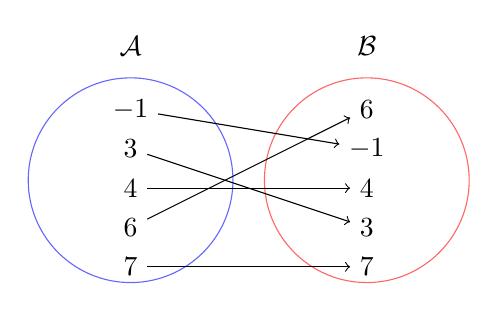
\begin{tikzpicture}
        % draw the sets
        \filldraw[fill=white!20, draw=blue!60] (-1.5,0) circle (1.3cm);
        \filldraw[fill=white!20, draw=red!60] (1.5,0) circle (1.3cm);


        % the texts
        \node at (-1.5,1.7) {$\mathcal{A}$};
        \node at (1.5,1.7) {$\mathcal{B}$};

        % the points in the sets (here I just create nodes to use them later on to position
        % the circles and the arrows
        \node (x1) at (-1.5,0.9) {$-1$};
        \node (x2) at (-1.5,0.4) {$3$};
        \node (x3) at (-1.5,-0.1) {$4$};
        \node (x4) at (-1.5,-0.6) {$6$};
        \node (x5) at (-1.5,-1.10) {$7$};
        \node (y1) at (1.5,0.9) {$6$};
        \node (y2) at (1.5,0.4) {$-1$};
        \node (y3) at (1.5,-0.1) {$4$};
        \node (y4) at (1.5,-0.6) {$3$};
        \node (y5) at (1.5,-1.10) {$7$};

        % draw the arrows
        \draw[->] (x1) -- (y2);
        \draw[->] (x2) -- (y4);
        \draw[->] (x3) -- (y3);
        \draw[->] (x4) -- (y1);
        \draw[->] (x5) -- (y5);

    \end{tikzpicture}
  \end{center}
  From the diagram we can see that no two elements from $\mathcal{A}$ are mapped to the same element in $\mathcal{B}$, hence
  $\operatorname{id}_\mathcal{A}$ is injective. Also since each element in $\mathcal{B}$ is mapped to, we conclude that
  $\operatorname{id}_\mathcal{A}$ is surjective. Hence $\operatorname{id}_\mathcal{A}$ is an invertible function.
\end{qstn}

\begin{qstn}
  \begin{solution}
    It is indeed true that  $\mathcal{R}_T = \mathcal{B}$. This is because if $T$ is invertible, then $T$ is surjective,
    if $T$ is surjective, then every element in $\mathcal{B}$ is mapped to, meaning that the set of all outputs for $T$ is $\mathcal{B}$,
    in other words, $\mathcal{R}_T = \mathcal{B}$.
  \end{solution}
\end{qstn}

\begin{qstn}
  \begin{solution}
    The following is the mapping diagram for $\mathcal{L}$,
    \begin{center}
     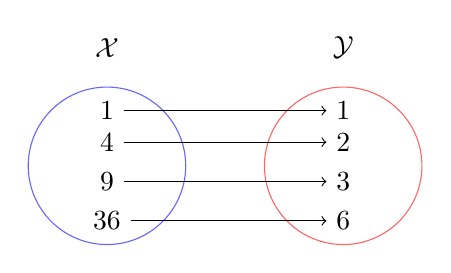
\begin{tikzpicture}
        % draw the sets
        \filldraw[fill=white!20, draw=blue!60] (-1.5,0) circle (1cm);
        \filldraw[fill=white!20, draw=red!60] (1.5,0) circle (1cm);


        % the texts
        \node at (-1.5,1.5) {$\mathcal{X}$};
        \node at (1.5,1.5) {$\mathcal{Y}$};

        % the points in the sets (here I just create nodes to use them later on to position
        % the circles and the arrows
        \node (x1) at (-1.5,0.7) {$1$};
        \node (x2) at (-1.5,0.3) {$4$};
        \node (x3) at (-1.5,-0.2) {$9$};
        \node (x4) at (-1.5,-0.7) {$36$};
        \node (y1) at (1.5,0.7) {$1$};
        \node (y2) at (1.5,0.3) {$2$};
        \node (y3) at (1.5,-0.2) {$3$};
        \node (y4) at (1.5,-0.7) {$6$};

        % draw the arrows
        \draw[->] (x1) -- (y1);
        \draw[->] (x2) -- (y2);
        \draw[->] (x3) -- (y3);
        \draw[->] (x4) -- (y4);

    \end{tikzpicture}
  \end{center}
  From the diagram we can see that no two elements from $\mathcal{X}$ are mapped to the same element in $\mathcal{Y}$, hence
  $\mathcal{L}$ is injective. Also since each element in $\mathcal{Y}$ is mapped to, we conclude that
  $\mathcal{L}$ is surjective. Hence $\mathcal{L}$ is an invertible function.
  \end{solution}
\end{qstn}

\begin{qstn}
  \begin{solution}
    The following is the mapping diagram for $\mathcal{P}$,
    \begin{center}
     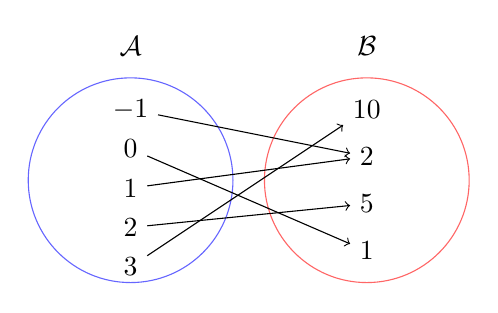
\begin{tikzpicture}
        % draw the sets
        \filldraw[fill=white!20, draw=blue!60] (-1.5,0) circle (1.3cm);
        \filldraw[fill=white!20, draw=red!60] (1.5,0) circle (1.3cm);


        % the texts
        \node at (-1.5,1.7) {$\mathcal{A}$};
        \node at (1.5,1.7) {$\mathcal{B}$};

        % the points in the sets (here I just create nodes to use them later on to position
        % the circles and the arrows
        \node (x1) at (-1.5,0.9) {$-1$};
        \node (x2) at (-1.5,0.4) {$0$};
        \node (x3) at (-1.5,-0.1) {$1$};
        \node (x4) at (-1.5,-0.6) {$2$};
        \node (x5) at (-1.5,-1.10) {$3$};
        \node (y1) at (1.5,0.9) {$10$};
        \node (y2) at (1.5,0.3) {$2$};
        \node (y3) at (1.5,-0.3) {$5$};
        \node (y4) at (1.5,-0.9) {$1$};

        % draw the arrows
        \draw[->] (x1) -- (y2);
        \draw[->] (x2) -- (y4);
        \draw[->] (x3) -- (y2);
        \draw[->] (x4) -- (y3);
        \draw[->] (x5) -- (y1);

    \end{tikzpicture}
  \end{center}
  Notice that since $\mathcal{P}(-1) = \mathcal{P}(1) = 2$, we conclude that $\mathcal{P}$ fails to be injective. Since
  $\mathcal{P}$ fails to be injective, it fails to be invertible.
  \end{solution}
\end{qstn}



\end{document}




























